%========================%
%        Preamble        %
%========================%
\documentclass[12pt]{amsart}

    %========================%
%        Packages        %
%========================%

\usepackage[utf8]{inputenc}
%\usepackage{amsmath}    % Included in amsart package
%\usepackage{amsthm}     % 
\usepackage{amssymb}      % 
\usepackage{mathtools}      % Paired Limiter Macros
% \usepackage{mdframed}       % boxes for theorem
\usepackage{enumitem}     % Continuous numbering of lists
\usepackage[hidelinks]{hyperref}
\usepackage{tikz}
\usetikzlibrary{positioning}
\usepackage{blindtext}
\usepackage{graphicx}
\usepackage{float}

%========================% 
%          Title         %
%========================% 
\title{Chapters 23 and 24 Notes}
\author{Anish Sundaram}
\date{\today}

%========================% 
%        Theorems        %
%========================% 
\theoremstyle{definition}
\newtheorem{theorem}{Theorem}  % Boxed theorems
\newtheorem{definition}{Definition} % Definitions
\newtheorem{example}{Example}       %
\newtheorem{algorithm}{Algorithm}
\newtheorem*{proof*}{Proof}         % non-numbered
\newtheorem*{remark}{Remark}        %
\numberwithin{equation}{theorem}    % Local equation numbering

\setcounter{tocdepth}{3}      % Show subsubsections in contents

%========================% 
%        Macros          %
%========================% 
\DeclarePairedDelimiter\abs{\lvert}{\rvert}  % Vertical bars
\DeclarePairedDelimiter\norm{\lVert}{\rVert} % Double vertical bars
\newcommand{\drawvec}[1]{                    % matrices on one line
    \begin{bmatrix}
        #1
    \end{bmatrix}
}


% \begin{figure}[H]
%     \centering
%     \includegraphics[width=5in]{global-carbon-cycle.png}
%     \caption{The Global Carbon Cycle}
%     \label{global-carbon-cycle}
% \end{figure}

%========================% 
%         Document       %
%========================% 
\begin{document}

\maketitle

\tableofcontents

\section*{23 Electric Potential}
When a charged particle moves in an electric field, the field exerts a force 
that can do work on the particle. This work can be expressed in terms of 
electric potential energy. Just as gravitational potential energy depends on 
the height of a mass above the earth’s surface, electric potential energy 
depends on the position of the charged particle in the electric field. 
In circuits, a difference in potential from one point to another is often 
called voltage. 

\subsection*{23.1 Electric Potential Energy}

\begin{definition}
    \textbf{Work done by a Force}: In non-electrical circumstances, the work
    done by a pushing force can be summarized as the exchange in energy by the
    force, and can be expressed by $$W_{a\rightarrow b} = \int^{b}_{a} \vec{f} \cdot d \vec{l} = \int ^b _a Fcos\phi dl $$
    where the force is positive if in same direction as movement.
\end{definition}

\begin{figure}[H]
    \centering
    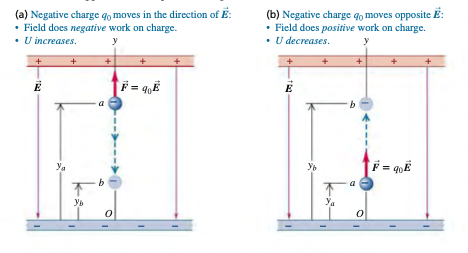
\includegraphics[width=5in]{Media/Work.png}
    \caption{Electric Field doing work on negative charge}
    \label{Electric Field doing work on negative charge}
\end{figure}



\begin{theorem}
    \underline{Work-Energy Theorem}: Work is defined as the negative of the
    change in \textit{potential energy}, in that a decrease in potential means an increase
    in energy through positive work. This can be expressed mathematically as 
    $$W_{a \rightarrow b} = -\Delta U$$ for the specific case the work is 
    conservative. This theorem also makes so \textit{Total Mechanical Energy} is conserved.
\end{theorem}

\begin{figure}[H]
    \centering
    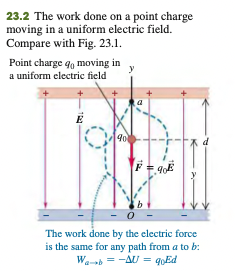
\includegraphics[width=5in]{Media/Conservative.png}
    \caption{Electric Field as Conservative Force}
    \label{Electric Field as Conservative Force}
\end{figure}


\subsubsection*{23.1.1 Electric Potential Energy in a Uniform Field}

\begin{definition}
    \textbf{Electric Potential Energy in a Uniform Field}:
    In the case of a uniform field, the value of the potential energy 
    can be described as $$U = q_0 E_y$$ where the value of $q$ depends on the charge
    and the sign of the potential energy depends on direction of travel, either
    along the electric field or opposite.
\end{definition}

\subsubsection*{23.1.2 Electric Potential Energy of Point Charges}

\begin{definition}
    \textbf{Electric Potential Energy of 2 point charges}:
    Expressed mathematicall as $$U = \frac{1}{4\pi\epsilon _0}\frac{qq_0}{r}$$
    Because potential energy is a shared property the relation is 1/r, also 
    noting that the sign of charges are kept as If $q$ and $q_0$ have the 
    same sign, the interaction is repulsive, this work is positive, and 
    U is positive at any finite separation. If the charges have opposite signs 
    the interaction is attractive and the work done is negative so U is negative. 
\end{definition}

\begin{definition}
    \textbf{Electric Potential Energy of Several Point Charges}:
    Because the Electric Potential of 2 points is a vector sum we can simply sum
    all the point charges together as path of travel does not matter for conservative
    forces. Thus our equation becomes $$U = \frac{q_0}{4\pi \epsilon _0} \Sigma _1 \frac{q_i}{r_i}$$
    \begin{remark}
        We can represent any charge distribution as a collection of point 
        charges, so it follows that for every electric field due to a static 
        charge distribution, the force exerted by that field is conservative.
    \end{remark}
\end{definition}


\begin{figure}[H]
    \centering
    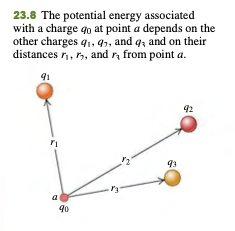
\includegraphics[width=5in]{Media/Potential.png}
    \caption{Potential Energy of Charges}
    \label{Potential Energy of Charges}
\end{figure}

\subsection*{23.2 Electric Potential}

\begin{definition}
    \textbf{Electric Potential}:
    Otherwise called just \textit{Potential}, this concept aids in determining
    involved energies of charged particles, and is defined as potential energy 
    per unit charge, and written mathematically as 
    $$ V = \frac{U}{q_0} \Leftrightarrow U = q_0V$$
    and has the SI unit of volt (V) or as joules/coulomb(J/C). When $U$ is expanded
    the equation becomes:
    \begin{enumerate}
        \item for a single point charge $$V = \frac{1}{4\pi\epsilon_0}\frac{q}{r}$$ 
        \item for multiple point charges $$V = \frac{1}{4\pi\epsilon_0} \Sigma_i \frac{q_i}{r_i}$$ 
        \item and for a continuous distribution of charge. $$V = \frac{1}{4\pi\epsilon_0} \int\frac{dq}{r}$$ 
    \end{enumerate} 
    \begin{remark}
        Potential Energy and Charge are both scalars, so Electric Potential 
        is also a scalar. 
    \end{remark}
\end{definition}



\begin{definition}
    \textbf{Voltage}:
    Voltage $V_{ab}$ is the potential (in Volts) of $a$ with respect to $b$,
    and equals the work (in Joules) done by the electric force when a 
    UNIT (1-C) charge moves from a to b.
\end{definition}


\subsubsection*{23.2.1 Electric Potential from Electric Field}
\begin{definition}
    \textbf{Electric Potential from Electric Field}:
    Because there is an easy conversion from force to Electric field in 
    $F = \vec{E}q$ we can simply substitute in $\vec{E}$ such that 
    $$V_a - V_b = - \int ^a _b \vec{E}\cdot d\vec{l}$$
    This also makes sense because the units match: 1 V/m = 1 volt/meter = 1 N/C = 1 newton/coulomb
\end{definition}

\begin{figure}[H]
    \centering
    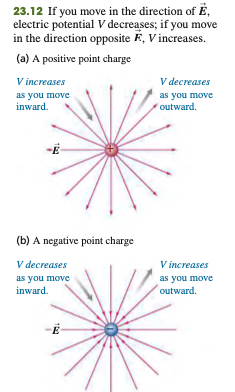
\includegraphics[width=5in]{Media/ElectricPotential.png}
    \caption{Electric Potential and Electric Field}
    \label{Electric Potential and Electric Field}
\end{figure}

\subsubsection*{23.2.2 Electron Volt}

\begin{definition}
    \textbf{Electron Volt}:
    The quantity of energy equivalent of a single electron with a potential difference
    of 1 V. 1eV = $1.602 * 10^{-19} J$
\end{definition}

\subsection*{23.4 Equipotential Surfaces}

\begin{definition}
    \textbf{Equipotential Surfaces}:
    In a similar manner to field lines, these surfaces are countout lines for 
    equal electric potential and emit radially from a charge. Potential along lines
    are equal and thus no work to go along. Lines close together indicate the field doing 
    large amounts of work in small displacement and $\vec{E}$ is large.
    \begin{remark}
        The electric field must always be perpendicular to the Equipotential 
        surface except in a uniform field where equipotential surfaces 
        are parallel planes perpendicular to field lines
    \end{remark}

    \begin{remark}
        When all charges are at rest, the surface of a conductor is always an 
        equipotential surface and the entire volume of a conductor is at equal potential
    \end{remark}

    \subsection*{23.5 Potential Gradient}

    \begin{definition}
        \textbf{Potential Gradient}:
        If the poten­tial V is known as a function of the coordinates x, y,
        and z, the components of electric field E at any point are
        given by partial derivatives of V:

        $$E_x = -\frac{\partial V}{\partial x},E_y = -\frac{\partial V}{\partial y},
        E_z = -\frac{\partial V}{\partial z}   $$ which in vector form produces 
        $$\vec{E} = -(\hat{i}\frac{\partial V}{\partial x} 
        +\hat{j}\frac{\partial V}{\partial y} 
        + \hat{k}\frac{\partial V}{\partial z} )$$
    \end{definition}

\end{definition}



\pagebreak

\section*{Important Equations}


\textbf{}

\textbf{}

\end{document}